%\documentclass{article} %[twocolumn] 
%\documentclass[Crown, times, sagev]{sagej}
\documentclass[sagev, Crown]{sagej}

%\usepackage{algorithmic}
\usepackage{algorithm}
\usepackage{algorithmicx}
\usepackage{algpseudocode}
\usepackage{booktabs}
\usepackage{array}
\usepackage{graphicx}
\usepackage{amsmath}
\usepackage{amsfonts}
\usepackage{amssymb}
\usepackage{multirow}
\usepackage{url}

\setcounter{secnumdepth}{3} %Gives section numbers for cross referencing
\begin{document}

\runninghead{Wilson et al.}

\title{Optimising error rates in pilot and definitive trial programmes using Bayesian statistical decision theory}

\author{Duncan T. Wilson\affilnum{1}}%,
%Rebecca E. A. Walwyn\affilnum{1}, 
%Julia Brown\affilnum{1} and 
%Amanda J. Farrin\affilnum{1}}

\affiliation{\affilnum{1}Leeds Institute of Clinical Trials Research, University of Leeds, Leeds, UK} %\\
%\affilnum{2}Centre for Primary Care \& Public Health, Queen Mary University of London, London, UK}

\corrauth{Duncan T. Wilson, Clinical Trials Research Unit, Leeds Institute of Clinical Trials Research, University of Leeds, Leeds, LS2 9JT, UK}
\email{d.t.wilson@leeds.ac.uk}

\begin{abstract}
% (300 word limit for ICTMC) (250 limit for SiM)
Pilot trials of complex interventions are often conducted in advance of a definitive trial to assess feasibility and to inform its design. Hypothesis tests of the efficacy of the intervention are rarely used in pilot trials due to the low power such a test would have, given the small sample size of a pilot and assuming a conventional type I error rate (e.g. 0.025). While increasing the type I error rate will increase power whilst maintaining a low sample size, there is little methodological guidance on how to balance these three factors. We consider a decision-theoretic approach to finding the optimal balance of type I and II error rates and sample size in pilot and definitive trial programmes. We introduce a general utility function which accounts for improvement in primary outcome, the cost of sampling, treatment costs, and the decision-maker's attitude to risk, with the optimal programme determined by maximising expected utility. We apply the method to the re-design of OK-Diabetes, a pilot trial with a continuous primary outcome with known standard deviation and where uncertainty in the treatment effect is quantified using a normal prior distribution. We then examine how optimal designs vary with the parameters of the utility function. We find that the decision-makers attitude to risk is an important factor in determining the optimal design, and that the conventional approach of not testing in a pilot trial can be optimal for highly risk-seeking decision makers.
\end{abstract}

\keywords{Clinical trial, pilot trial, external pilot, statistical decision theory, optimal design}

\maketitle

\section{Introduction}

Pilot trials are a type of feasibility study \cite{Eldridge2016} commonly conducted prior to large, definitive complex intervention trials to assess their feasibility and inform their design \cite{Craig2008}. Taking the same form as the planned definitive trial but on a smaller scale, they may be \emph{external} or \emph{internal}. An external pilot's data is kept separate from the definitive trial's, with a clear gap between the two stages; whereas an internal pilot's data will be used as part of the final analysis, with a seamless gap between. Whether internal or external, a key goal of any pilot is to guide the decision of whether or not the definitive trial should go ahead.

A common theme which has emerged in the methodological pilot literature is that pilot trials should be clearly distinguished by their aims, which are to inform the feasibility and optimal design of a planned definitive trial \cite{Lancaster2004, Arain2010, Thabane2010, Eldridge2016, Eldridge2016a}. In particular, it has been noted that pilots are not designed to assess the effectiveness of the intervention, and as such any hypothesis tests of effectiveness are likely to be underpowered and should therefore be avoided \cite{Wilson2015}. This criticism rests on two assumptions. Firstly, it assumes that the pilot and definitive trials will share a primary endpoint with the same minimal clinically important difference (MCID). Secondly, it assumes that any pilot trial hypothesis test will be conducted at a conventional significance level, with a type I error rate in the range 0.01 - 0.1. For example, an external pilot trial designed using the rule-of-thumb of 35 participants per arm \cite{Teare2014} would have a power of 23\% to detect a standardised effect size of 0.3 when using a one-sided type I error rate of $\alpha = 0.025$.

While the assumption of a constant MCID will often hold\footnote{The case of phase II drug trials is a notable exception. There, it is common for the pilot to measure a short term binary response endpoint while the definitive trial will measure a long term survival endpoint. Thus, in the phase II setting, a larger MCID can be stated to be of interest and a small sample size can be reported as leading to conventionally small error rates.}, there is no obvious reason for type I error rates in pilots to be constrained at conventionally low levels. Indeed, by rejecting a possible pilot test with error rates $\alpha = 0.025$ and $\beta = 1 - 0.23 = 0.77$ and instead not testing at all, we effectively obtain a procedure with error rates $\alpha = 1, \beta = 0$. This decision reflects an infinite preference for minimising type II errors over type I errors in the pilot, a preference too extreme to be expected in practice. Even if the magnitude of preference is substantial, any finite level would lead to a different choice. For example, an alternative would be $\alpha = 0.9, \beta = 0.006$. In many cases we might expect a decrease in type I error of 0.1 in exchange for an increase in type II error of 0.006 to be a reasonable trade-off. Relaxing the type I error rate in pilot trials has been suggested explicitly \cite{Lee2014} and implicitly \cite{Cocks2013} before, although in neither case are methods for choosing an appropriate level described. More widely, it has been argued that conventional default choices for error rates should be avoided, choosing levels with regard to the problem and hand and providing justification for these choices \cite{Lakens2018, Bacchetti2019}.

\begin{figure}
\centering
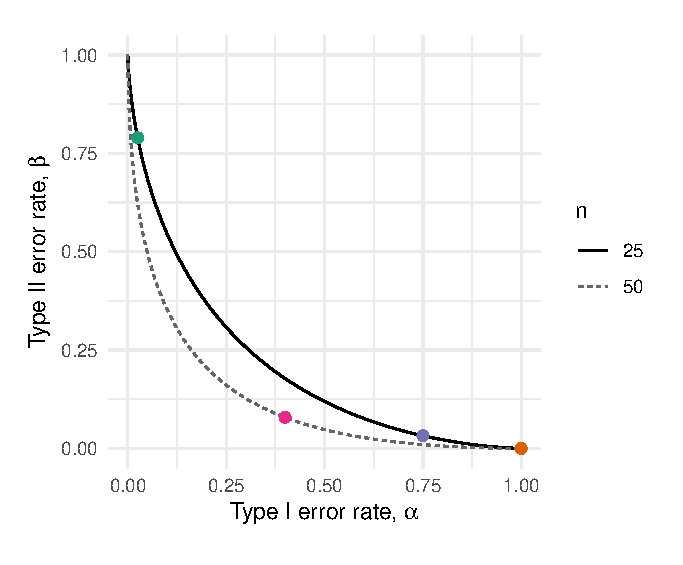
\includegraphics[scale=0.8]{./figures/ocs.eps}
\caption{Operating characteristic curves for an external pilot trial testing efficacy.}
\label{fig:ocs}
\end{figure} 

The question which we will consider in this paper is how to determine the optimal error rates for a test of effectiveness in a pilot trial which will be conducted prior to a definitive trial and used to guide the progression decision. One possible approach to defining such optimal decisions is Bayesian statistical decision theory. Under this framework we define a suitable utility function which encodes our preferences and make decisions based on the expected value of this utility with respect to a prior distribution which expresses our uncertainty on 
the unknown parameters. Although the theory is well established \cite{Raiffa1961, Keeney1976} and has been frequently proposed in methodological work around optimal trial design \cite{Lindley1997, Hee2016}, it has been argued that the requirement of specifying a utility function has led to low uptake in practice \cite{Joseph1997a}. 

One goal of this paper is to propose a simple and quite general form for a utility function in clinical trials, making clear the assumptions which are encoded and thus making it easy for the user to judge its applicability or otherwise to the problem at hand. The utility we propose is closely related to several existing proposals in the literature \cite{Pearce2018 ...}, but with some key differences. One particularly important aspect we have considered is the decision-makers attitude to risk, an issue sidestepped by many exiting proposals which assume, explicitly or implicitly, that the decision-maker is risk-neutral. We will show that the attitude to risk has a significant effect on decision making, and is key to answering one of the motivating questions of this paper: in what situations, if any, is it optimal to not test effectiveness in a pilot trial?

The remainder of this paper is structured as follows. We define the specific problem under consideration in Section \ref{sec:problem}, and then provide the necessary background regarding Bayesian statistical decision theory in Section \ref{sec:bsdt}. The prosed method is described in Section \ref{sec:methods}. In Section \ref{sec:illustration} we illustrate the application of the method to design an external pilot of a complex intervention.

% Ref to VoI lit

\section{Problem}\label{sec:problem}

We consider the problem of jointly designing an external pilot trial and subsequent definitive trial. We will denote these, respectively, as stages $i=1$ and $i=2$ of the overall programme. We consider the case where both trials are parallel group studies comparing an intervention to control. We assume that the comparison focusses on superiority in terms of the mean difference of a normally distributed primary endpoint with known standard deviation common to each arm, where the same endpoint is used in both the pilot and definitive trials (although see Section \ref{sec:extensions} for relaxations of some of these assumptions). 

We denote the true mean difference by $\mu$, and consider the case where the the primary analysis at each stage will be a test of the null hypothesis $H_0: \mu = 0$. The test at stage $i$ will compare the sample mean difference between groups, denoted  $x_i$, to a pre-specified critical value, denoted $d_i$. At the pilot stage, a positive result (i.e. $x_1 > d_1$) will indicate that we should proceed to the definitive trial. At the definitive stage, a positive result (i.e. $x_2 > d_2$) will indicate that the intervention should be recommended for use over the control treatment. The thresholds $d_1, d_2$, along with the per-arm sample sizes at each stage $n_1, n_2$, collectively define the design of the overall programme. The design problem we consider in this paper is to optimise $n_i, d_i, i = 1,2$.

Given some alternative hypothesis $H_1: \mu =\mu^*$, we define the type I and II error rates for stage $i$ in the usual way, i.e. $\alpha_i = Pr[x_i > d_i \mid \mu = 0]$ and $\beta_i = Pr[x_i \leq d_i \mid \mu = \mu^*]$. An alternative summary of the pilot and definitive trial programme is then  $\alpha_i, \beta_i, i=1,2$.

% to add - full, explicit likelhood model

\section{Bayesian statistical decision theory}\label{sec:bsdt}

A short review of the basics of Bayesian decision theory, with signposts to the relevant literature.

\section{Maximising expected utility in trial programmes}\label{sec:methods}

We consider a Bayesian view of the frequentist design problem, and therefore require prior distributions to be specified for the unknown true mean difference $\mu$. This prior information will be used only to guide the choice of the frequentist design and analysis parameters, and not in any analysis of the trial data itself. As such, a non- or weakly-informative prior is not appropriate; rather, the prior should be a subjective summary of the decision-maker's knowledge and uncertainty about $\mu$. For computational tractability we will assume a conjugate normal prior $p(\mu)$ with mean $m_0$ and variance $s^2$.

We define optimal design variables as those which maximise the expectation, with respect to the prior $p(\mu)$, of a utility function. We construct the utility function in three steps, following the procedures described by Keeney and Raiffa \cite{Keeney1976}. First, we identify the attributes which we consider will be of interest to the decision maker. We then define a value function over the space of these attributes, which encodes the decision-maker's preferences under conditions of certainty. We then transform this value function into a utility function by incorporating the decision-maker's attitude to risk. Throughout, we will make explicit the assumptions which are implied by the parametric forms of the value and utility functions, returning to discuss their implications in Section \ref{sec:discussion}.

\subsection{Attributes}

The average treatment outcome in the patient population will be determined by the trial results, the true treatment difference $\mu$, and the manner in which patients adopt the new treatment if it is made available. Considering the latter would require a model to predict how patients will choose treatments, and although this has been attempted in similar work \cite{Gittins2000a, Kikuchi2009} we will use a simple model assuming that the whole population will adopt the new treatment if the result of the definitive trial is positive, otherwise retaining the control treatment. So, our first attribute is the change in average outcome which we denote by $d$.

The sample size at both stages of the programme is of interest, being associated with both monetary costs and the exposure of patients to research. Sample size will vary from programme to programme, both by design and through the uncertain outcome of the pilot trial. If we consider sampling at each stage to be equivalent in terms of the costs involved, we can then identify the total sample size $n = n_1 + n_2$ as our second attribute. 

While the focus of comparison between the new treatment and control is on the primary outcome, the treatments will in general differ in other aspects. We limit ourselves to the case where these differences are deterministic, such as in treatment costs. In this case, we can encapsulate these differences in a single indicator variable, and our third attribute,  $C \in \{0, 1\}$ where $C = 0$ if and only if a positive result is obtained in the definitive trial. 

\subsection{Value}

We use the notation $y \prec y'$ to mean we prefer $y$ to $y'$, where $\prec$ is a weak ordering (i.e. complete and transitive) of all possible values $y$. We aim to specify a value function $v(n, C, d)$ such that
$$
(d, n, C) \prec (d', n', C') \Leftrightarrow v(d, n, C) < v(d', n', C').
$$
We will use a value function with the following additive form:
$$ 
v(d, n, C) =  v_d(d) + v_n(n) + v_c(C),
$$
where $v_n, n_c$ and $v_d$ are single-attribute value functions. It has been shown that such an additive value function exists if and only if the three attributes are pairwise preferentially independent (DEFINE). For example, this requires that attributes $\{n, C\}$ are preferentially independent of attribute $d$, in the sense that conditional preferences on the $(n, C)$ space given $d'$ d not depend on the specific value of $d'$; and likewise for the other two pairs.

We assume that the cost of sampling is constant, and so $v_n$ is linear, and similarly assume linearity in the value of change in outcome, $v_d$. Attribute $C$ only has two levels and therefore $v_c$ does not require any further specification. For ease of notation we will use the following single-attribute value functions:
$$ 
v_d(d) = k_d d, ~ v_n(n) = k_n n, ~ v_C(C) = k_c C.
$$
We deduce the parameter values as follows. First, we ask for the change in outcome $\bar{d}$ that would be needed for us to judge that
$$
(d = 0, n = 0, C = 1) \sim (d = \bar{d}, n = n_*, C = 1).
$$
That is, what change in outcome would we want to see to justify an increase in sample size from 0 to $n_*$? Note that the linear nature of $v_n$ and $v_d$ mean the specific choice of $n_*$ is arbitrary. Secondly, we ask for the change in outcome $\hat{d}$ that would be needed to judge that
$$
(d = 0, n, C = 1) \sim (d = \hat{d}, n, C = 0).
$$
That is, what change in outcome would justify moving from the current standard to the new treatment? Finally, since value functions are invariant under re-scaling, we can set $k_n + k_c + k_d = 1$ and therefore have the following system of three equations:
\begin{align*}
k_d \bar{d} + k_n n_* &= 0 \\
k_d \hat{d} - k_c &= 0 \\
k_d + k_n + k_c &= 1
\end{align*}
Solving this gives the following values for the scaling parameters:
\begin{equation}\label{eqn:ks}
k_d = 1/(1 + \hat{d} - \bar{d}/n_*), ~ k_n = -k_d \bar{d}/n_* , ~ k_c = k_d \hat{d}. 
\end{equation}



\subsection{Utility}

The value function represents our preferences under conditions of certainty, but in reality we are uncertain about the true values of all three attributes. To accommodate this uncertainty, we move from a value function to a utility function, where the latter encodes our preferences under uncertainty. A utility function allows us to compare probability distributions over the attributes, as opposed to only fixed points, and thus make decisions by choosing the distribution which has the largest expected utility.

To define the form of our utility function, we first argue that the change in outcome is \emph{additively independent} (DEFINE) of the other two attributes. This means that our preferences for gambles on the change of outcome, with the other attributes kept fixed at some level, does not depend on those levels. So, regardless of how much we have sampled, or whether or not we have incurred the cost of changing the standard treatment or not, our preferences for gambles on the change in outcome will be the same. Given this assumption together with the additive form of the value function, the utility function must have one of the following\cite{French2000} forms:
$$
u(n, C, d) =
\begin{cases}
1 - e^{-\rho v(n, C, d)}, &\rho > 0 \\
v(n, C, d), &\rho = 0 \\
-1 + e^{-\rho v(n, C, d)}, &\rho < 0 
\end{cases}
$$
Given the value function, the utility function is then fully defined by $\rho$. A value of $\rho = 0$ implies a risk-neutral attitude, whereas $\rho$ greater than (less than) 0 implies a risk-averse (risk-seeking) attitude. 

To elicit $\rho$ we first note that we can think about gambles on $d$ whilst ignoring the value of the other attributes since $d$ is utility independent of $n$ and $C$. For a given value of $\rho$ we then consider the value $d^*$ such that we would be indifferent between a) obtaining $d^*$ with certainty, and b) a gamble which will result in $d_{min}$ with probability 0.5 and $d_{max}$ with probability 0.5. That is, we find $d^*$ such that
$$
u(n, C, d^*) = 0.5u(n, C, d_{min}) + 0.5u(n, C, d_{max}).
$$
In the special case of risk-neutrality, $\rho = 0 \Leftrightarrow d^* = 0.5d_{min} + 0.5d_{max}$. For $\rho \neq 0$ we have
$$
d^* = - \frac{1}{\rho} \ln\left( 0.5e^{-\rho d_{min}} + 0.5e^{-\rho d_{max}} \right),
$$
and so we can determine $\rho$ given $d^*$. For example, setting (arbitrarily) $d_{min} = 0, d_{max} = 1$, a value of $\rho = 2$ corresponds with $d^* =  0.283$. That is, $\rho = 2$ implies an indifference between obtaining a guaranteed change in outcome of 0.283 and a simple 50/50 gamble between no change at all and a change of 1. 

%To find the exact value of $\rho$ for the problem at hand, we could plot the function $d^*(\rho)$ over a range of $\rho$.

\subsection{Expected utility}

Denote by $G_i \in \{0, 1\}$ an indicator variable where $G_i = 1$ if and only if there is a positive test result at stage $i = 1,2$. For the problem considered here, $G_i = 1 \Leftrightarrow x_i > d_i$. Noting that the attributes $D$, $n$ and $C$ are completely determined by the fixed programme design $z$, the realisations of $G_i, i=1,2$, and the true treatment effect $\mu$, we re-write utility as $u(\mu, G_1, G_2 ~|~ z)$. Focussing on the case where $\rho > 0$ (the other cases will follow), we have
\begin{equation}
\begin{split}
u(\mu, G_1, G_2 ~|~ z) = 1 - \exp(&-\rho[k_d\mu + k_n (n_1+n_2)] G_1 G_2 \\ 
  &- \rho[k_n (n_1+n_2) + k_c] G_1 (1 - G_2) \\
  &- \rho[k_n n_1 + k_c] (1 - G_1) ),
\end{split}
\end{equation}
The expected utility conditional on $\mu$ is
\begin{equation}\label{eqn:joint_cond_util}
\begin{split}
E_{G_1, G_2, | \mu, z}[u(\mu, G_1, G_2 ~|~ z)] =& Pr[G_1 = 1, G_2 = 1  \mid \mu]\left(1-e^{\rho(k_d\mu + k_n(n_1+n_2)}\right) + \\
& Pr[G_1 = 1,  G_2 = 0  \mid \mu] \left(1- e^{-\rho(k_n (n_1+n_2) + k_c)} \right) + \\
& Pr[G_1 = 0 \mid \mu] \left( 1-e^{-\rho(k_n n_1 + k_c)} \right),
\end{split}
\end{equation}
Since the sample means are distributed as $x_i \mid \mu \sim N(\mu, 2\sigma^2/n_i)$ and are independent conditional on $\mu$, the relevant conditional probabilities are easily calculated. We are then left with integrating out the unknown true treatment difference $\mu$, giving
\begin{equation}\label{eqn:exp_util}
E[u(\mu, G_1, G_2 ~|~ z)] = \int E_{G_1, G_2, | \mu, z}[u(\mu, G_1, G_2 ~|~ z)] p(\mu) d\mu.
\end{equation}

Because we are integrating with a normal density weighting function, we use Gauss-Hermite quadrature (as implemented in the `fastGHQuad` R package \cite{Blocker2018}) to evaluate the integral efficiently and accurately. %Specifically, Gauss-Hermite approximates integrals of the form
%$$
%\int_{-\infty}^{\infty} e^{-x^2}f(x) dx \approx \sum_{i=1}^{n} w_i f(x_i).
%$$
%To use when integrating over a normal distribution $y \sim N(\mu, \sigma^2)$, we use the transform $y = \sqrt{2}\sigma x + \mu$ so the integration points are now $x_i\sqrt{2}\sigma + \mu$ and the weights are $w_i / \sqrt{\pi}$.
For the special case where pilot trial operating characteristics are fixed at $\alpha_1 = 1, \beta_1 = 0$, the exact expected utility can be derived and numerical integration can be avoided. Full details are given in the appendix.


\subsection{Optimisation}\label{sec:optimisation}

Optimal programme designs can be found by solving the optimisation problem
\begin{alignat}{1}\label{eqn:opt}
\max_{z = (n_1, d_1, n_2, d_2)} ~ & E[u(\mu, G_1, G_2 ~|~ z)] \\
\text{subject to} ~ & n_i \in \mathbb{N}, i=1,2, \nonumber \\ 
& d_i \in \mathbb{R}, i=1,2. \nonumber
\end{alignat}
We first apply the global optimisation algorithm DIRECT \cite{Jones1993}, and then use the resulting solution as the starting point for the Subplex local optimisation algorithm \cite{Rowan1990}. Both of these algorithms are implemented in R via the package `nloptr' \cite{Ypma2018}. Full details are provided in the supplementary material.

%We use a standard particle swarm algorithm \cite{Clerc2012} as implemented in the R package `pso' \cite{Bendtsen2012}. Fast and reliable optimisation is obtained by supplying the partial derivatives of the expected utility function, as described in the appendix.

\section{Illustration}\label{sec:illustration}

%We consider the hypothetical problem described by Stallard (20012)\cite{Stallard2012}, where a pilot trial is to be conducted prior to a planned definitive trial with a shared normally distributed primary endpoint, known standard deviation of $\sigma = 1$, and an MCID of $\delta = 1$. The true treatment effect $\mu$ has a normal prior with $\mu_0 = 0, \sigma_0 = 1$. Note that this represents an archetypal sceptical view of the treatment effect \cite{Spiegelhalter1993}, and that it implies a prior belief that the effect will be greater than the MCID with probability 0.159. These parameters mean that a definitive trial designed to have conventional error rates of 0.025 and 0.1 would require a sample size of 21 in each arm.

OK-Diabetes \cite{Walwyn2015} aimed to assess the feasibility of evaluating supported self-management for adults with learning disabilities and type II diabetes. The original target sample size was 30 patients per arm, chosen based on a rule-of-thumb \cite{Lancaster2004} and to allow the feasibility objectives of the study to be addressed. The team were asked by the funder to consider assessing the potential efficacy of the intervention to determine whether a seamless confirmatory trial should go ahead. A continuous measure of participant blood sugar levels (HbA1c) at six months was chosen as the efficacy outcome. The SD of this outcome was identified to be 1.5\% \cite{OKD2013}. A mean change of 0\% was considered to be of no interest, whilst a mean reduction of 0.5\% at six months 6 months was deemed clinically important. The target sample size was increased to 56 participants per arm, giving $1-\beta_1 = 0.82$ power to detect a true mean reduction of 0.5\% using a one-sided test with a type I error rate of $\alpha_1 = 0.2$. Although the error rates for the subsequent definitive trial were not specified, we note that a sample size of 190 participants per arm would lead to $1-\beta_2 = 0.9$ power to detect a true mean reduction of 0.5\% using a conventional one-sided type I error rate of $\alpha_2 = 0.025$. Here, we consider how the proposed method could be used to determine optimal choices of $\alpha_i, \beta_i, i=1,2$.

To apply the proposed method we require a prior distribution on the treatment difference and a utility function. For the former, we use a conjugate normal prior with parameters $m_0 = 0$ and $s_0 = 0.6$. This represents a sceptical prior, being centred at the null hypothesis of no difference and with a variance corresponding to a prior belief that $\mu > \mu_1 = 0.5$ with probability 0.20.

For the utility function, we first consider the change in outcome which would be enough to justify the costs of switching from the current standard treatment to the new treatment under study. To determine this value we first assume that the above conventional design with a type I error rate of 0.025 and a power of 0.8 to detect $\mu = 0.5$ is an approximate reflection of the decision-maker's preferences. This design would lead to 0.5 power when $\mu = 0.3$, implying that we would be indifferent between adopting the new treatment and staying with the current standard if this was the true treatment difference \cite{Willan2005}. This gives a rationale for choosing $\hat{d} = 0.3$. For the cost of sampling, we need to identify a change in treatment which would justify an increase in sample size from 0 to $n_* = 50$ (recall that the choice of $n_*$ is arbitrary). For the purposes of illustration we suppose that this leads to $\bar{d} = 0.005$, meaning that we consider an increase in sample size of 50 to be worthwhile if we obtained a guaranteed change in treatment effect of 0.005. %Note that these two values, together with the additive form of the value function, imply the value judgement
%$$
%(n = 0, C = 1, d) \sim (n = \hat{d}n_*/\bar{d} = 3000, C = 0, d).
%$$
%That is, under conditions of certainty, we would judge the costs of switching from the standard treatment to be equal to the cost of recruiting and following up 3000 patients in each arm. 
Given these judgements and using equation \ref{eqn:ks}, we have the value function
$$ 
v(d, n, C) = 0.769 d - 0.0000769 n + 0.231 C.
$$
Moving to utility, we set $d_{min} = 0$ and $d_{max} = 0.5$ (arbitrarily) and consider the change of treatment we would like to obtain for certain for it to be judged equivalent to a simple 50/50 gamble between $d_{min}$ and $d_{max}$. We suppose a risk-averse attitude leads to $d^* = 0.19$, corresponding to $\rho = 2$. Our utility function is then
$$
u(d, n, C) = 1 - \exp[ - 2 \times (0.769 d - 0.0000769 n + 0.231 C)].
$$
Given the prior and utility parameters, we now consider two variations of the optimal design problem. First, we optimise jointly over the pilot and main trial programme (`unrestricted'). Then, we optimise only the main trial whilst fixing $\alpha_1 = 1, \beta_1 = 0$ (`no pilot test'). The algorithm takes around 1 second to converge to a solution in the general unrestricted case. For the special case of no pilot test where an exact expression of expected utility is available, convergence takes around 0.003 seconds. The results are given in Table \ref{tab:ill}. 

\begin{table}
\small\sf\centering
\caption{Optimal sample size and error rates for the OK-Diabetes external pilots trial ($i = 1$) and subsequent definitive trial($i = 2$), both for the general unrestricted case and where we insist on not testing effectiveness in the pilot trial.}
\input{./tables/ill.txt}
\label{tab:ill}
\end{table}

In the unrestricted case we find that the optimal programme involves an external pilot sample size of $n_1 = 41$ participants per arm, between the initial and revised choices of sample size of 30 and 56 used in OK-Diabetes. The balance of error rates in the pilot is, however, substantially different to those chosen previously. We find that a considerable type I error rate of $\alpha_1 = 0.51$ is used, allowing a high power of $1-\beta_1 = 0.938$ whilst maintaining a low sample size. Having allowed a large type I error rate in the pilot, the optimal definitive trial uses $\alpha_2 = 0.012$, around half the conventional choice of 0.025. 

In comparison, when we insist on not testing in the external pilot we obtain a lower definitive trial sample size of $n_2 = 135$, with more conventional error rates of $\alpha_2 = 0.02$ and $1 - \beta_2 = 0.755$. The expected utility of this programme is 0.00126 lower than the optimal unrestricted programme. To interpret this, we can translate utilities back to values and then into attribute units. Specifically, this difference in utility corresponds to a difference in value of
$$
\log(1-0.42558) - \log(1-0.42874) = 0.005516389,
$$
and dividing this by $k_n$ leads to an effective difference of 72. That is, we can consider the unrestricted optimal design to be more efficient than the restricted design by an amount equivalent to recruiting and following up 72 participants.

%\subsection{Sensitivity analysis}

Having obtained an optimal programme design for a certain choice of prior and utility parameters, it is of interest to assess how robust this design is to deviations from these. To do this we consider a range of alternative parameter values and, for each, determine the optimal programme design. The expected utility of this optimal design can then be compared against that of the proposed design, converted into units of sample size as above. We will refer to this difference as the \emph{regret}. We conducted two sensitivity analyses: first, we varied the prior parameters $m_0$ and $s_0$; secondly, we varied the utility parameters $\rho$ and $\bar{d}$. All other parameters were kept at their original values.

\begin{figure}
\centering
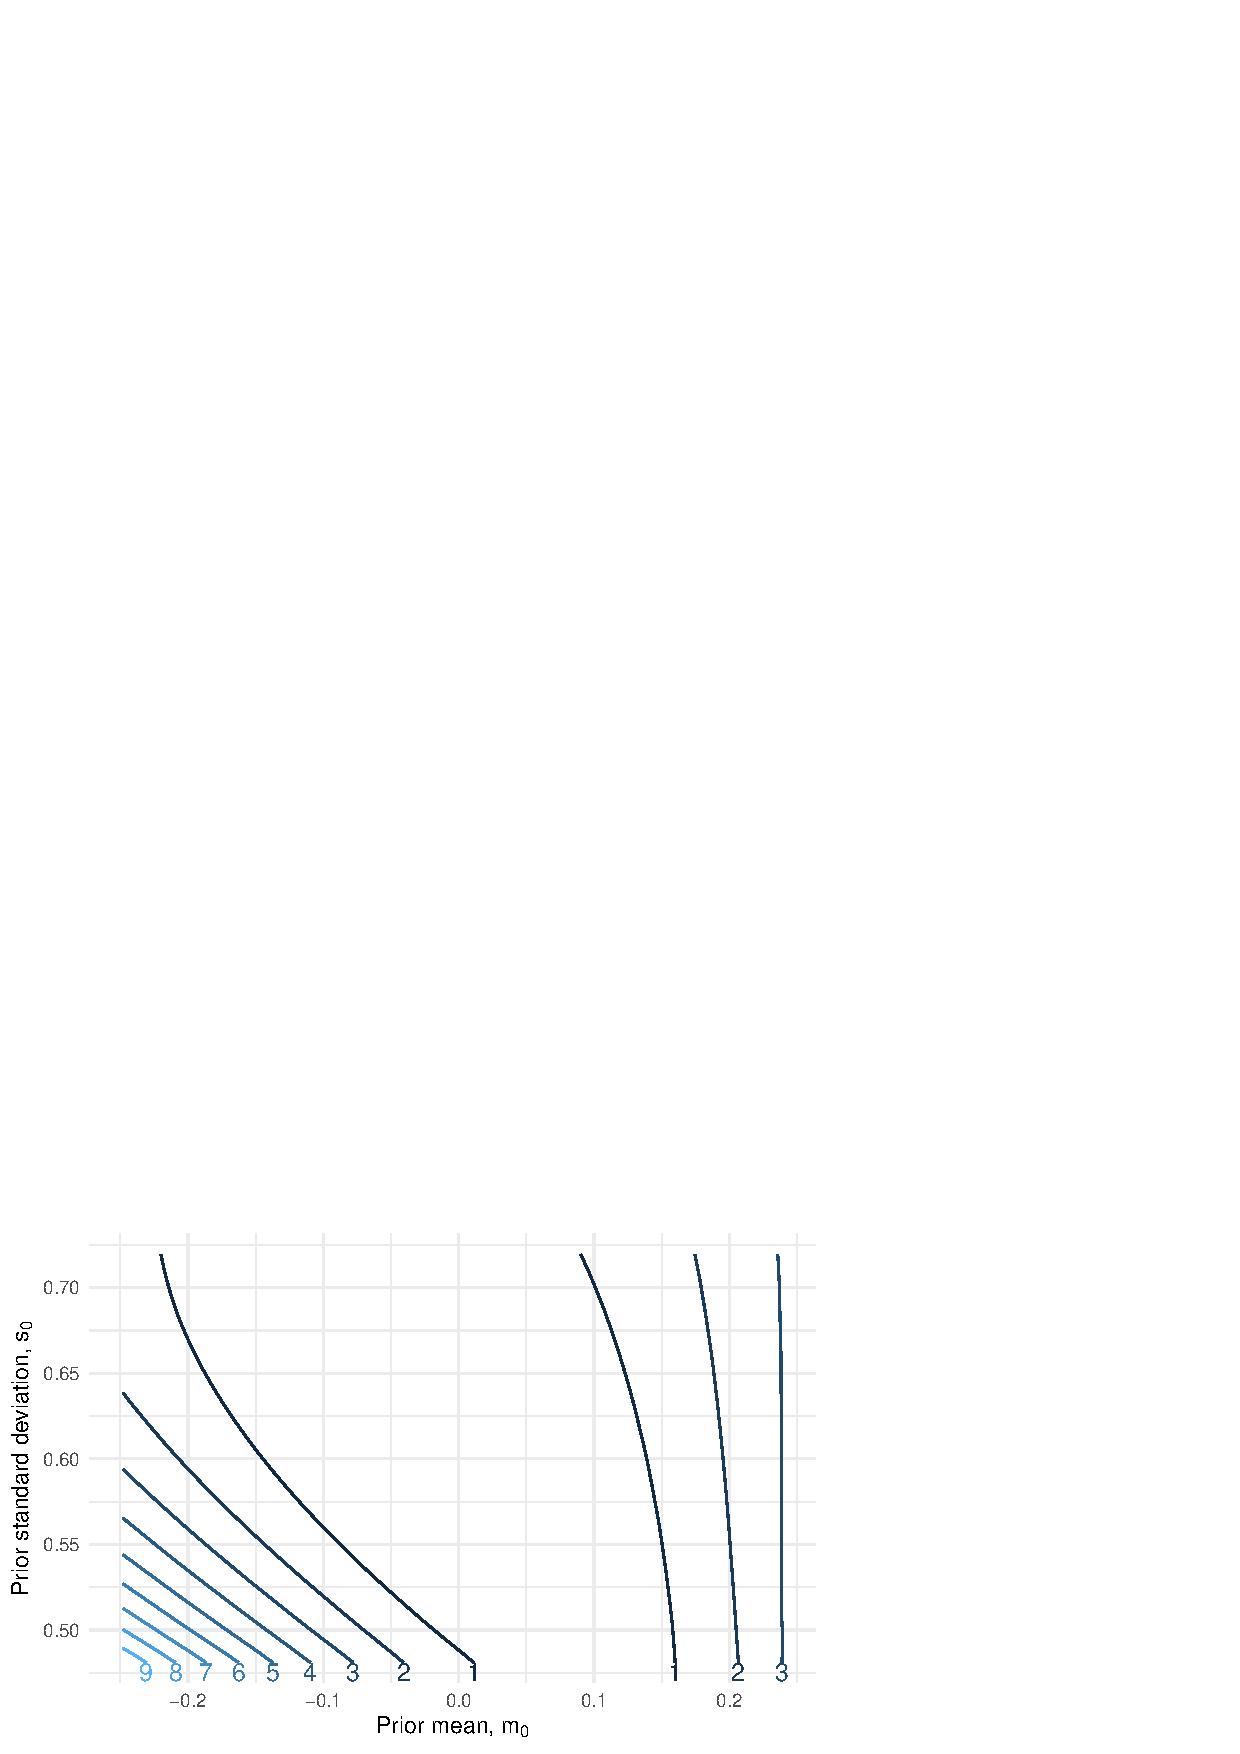
\includegraphics[scale=0.8]{./figures/sens_p.pdf}
\caption{Amount of regret when using the proposed OK-Diabetes programme design as the prior mean $m_0$ and prior standard deviation $s_0$ vary. Contours are generated by fitting a generalised additive model with tensor product smooth term to a 500 point space-filling Sobol sequence experimental design.}
\label{fig:sens_p}
\end{figure} 

Figure \ref{fig:sens_p} plots the regret over a range of prior means $m_0$ and prior standard deviations $s_0$. We varied the prior mean from -0.5 to 0.5, moving from extremely sceptical to enthusiastic beliefs. We find that over this range there is
 little to be gained from moving from the proposed design to the optimum, providing the prior standard deviation is equal to or less than the initial choice of $s_0 = 1$. As we increase $s_1$ up to 1.2, the penalty of using the proposed design can increase, but the magnitude of these penalties depends also on $m_0$. From these results we can conclude that the proposed design is quite robust to misspecification of the prior distribution in the sense that if the choices of $m_0, s_0$ are not quite an accurate reflection of our prior beliefs, the design will still have an expected utility close to that of the locally optimal design.

\begin{figure}
\centering
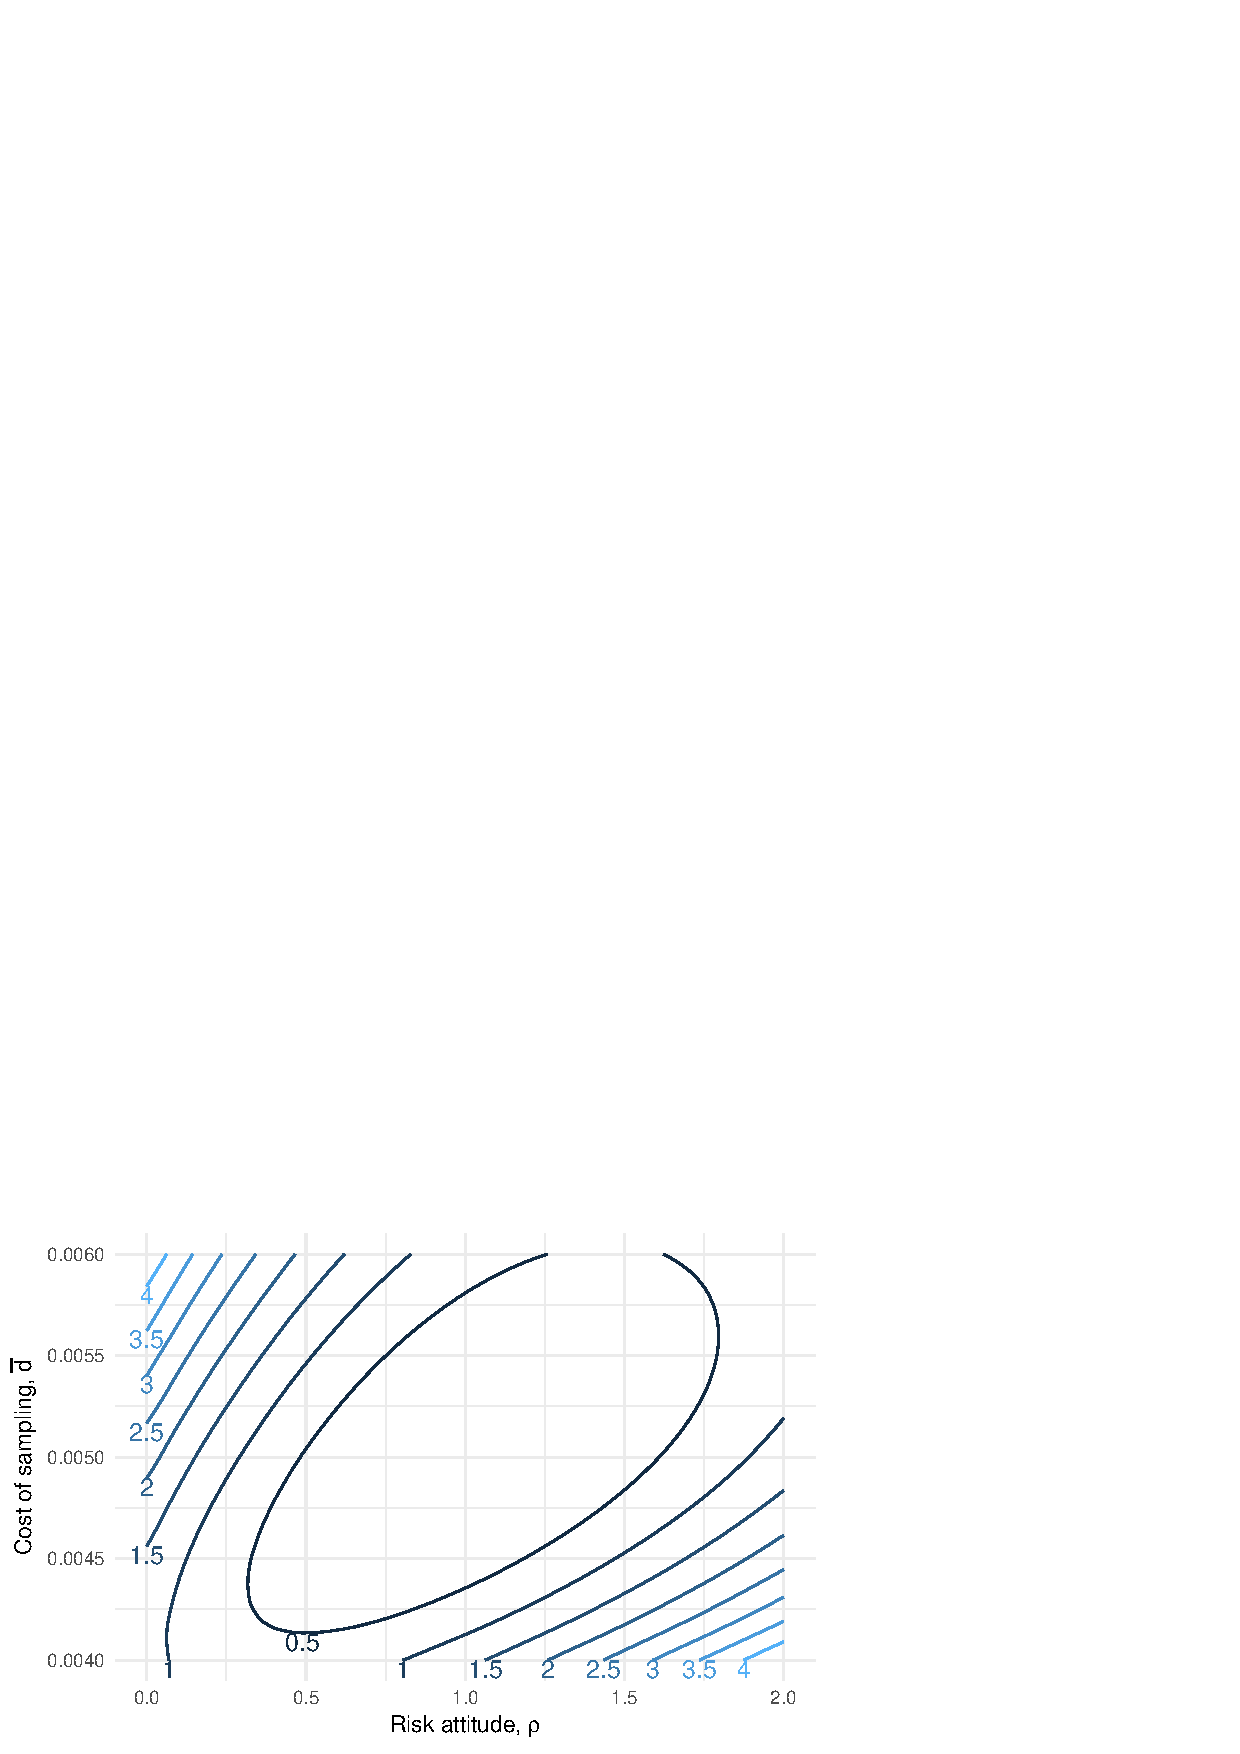
\includegraphics[scale=0.8]{./figures/sens_u.pdf}
\caption{Amount of regret when using the proposed OK-Diabetes programme design as the attitude to risk $\rho$ and cost of sampling $\bar{d}$ vary. Contours are generated by fitting a generalised additive model with tensor product smooth term to a 500 point space-filling Sobol sequence experimental design.}
\label{fig:sens_u}
\end{figure}

Corresponding results for varying utility parameters $\rho$ and $\bar{d}$ are given in Figure \ref{fig:sens_u}. Here we see that the proposed design is generally again quite robust to misspecification, except in one direction. If the true utility parameters reflect a more risk averse attitude (i.e. $\rho > 1$) \emph{and} a lower cost of sampling (i.e. $\bar{d} < 0.0025$), the proposed design can become considerably sub-optimal. For example, at the extreme point in the ranges we considered, with $\rho = 2, \bar{d} = 0.0015$, the difference in expected utility between the proposed and locally optimal designs are equivalent to over 24 participants. These sensitivity analyses suggest that the choice of $\bar{d}$ and $\rho$ in particular should be examined to ensure they are a true reflection of the decision-maker's preferences.


\section{Evaluation}\label{sec:evaluation}

In the preceding example we found that the standard policy of not testing for efficacy in an external pilot trial can be considerably sub-optimal. Here, we investigate the extent to which this holds as we vary the parameters defining the utility function. Throughout, we maintain the same archetypal sceptical prior with $m_0 = 0$ and $s_0 = 1$, and keep the treatment cost parameter at $\hat{d} = 0.3$ as before. We then varied both the attitude to risk, with $\rho \in [-5, 5]$, and the cost of sampling, with $\bar{d} \in [0.001, 0.01]$. For each $(\rho, \bar{d})$ pair we found the optimal programme. The results are given in Figure \ref{fig:eval}, which plots how the sample size and error rates of both the pilot ($i = 1$) and definitive ($i = 2$) trials vary with $\rho$, for six specific choices of $\bar{d}$.

\begin{figure}
\centering
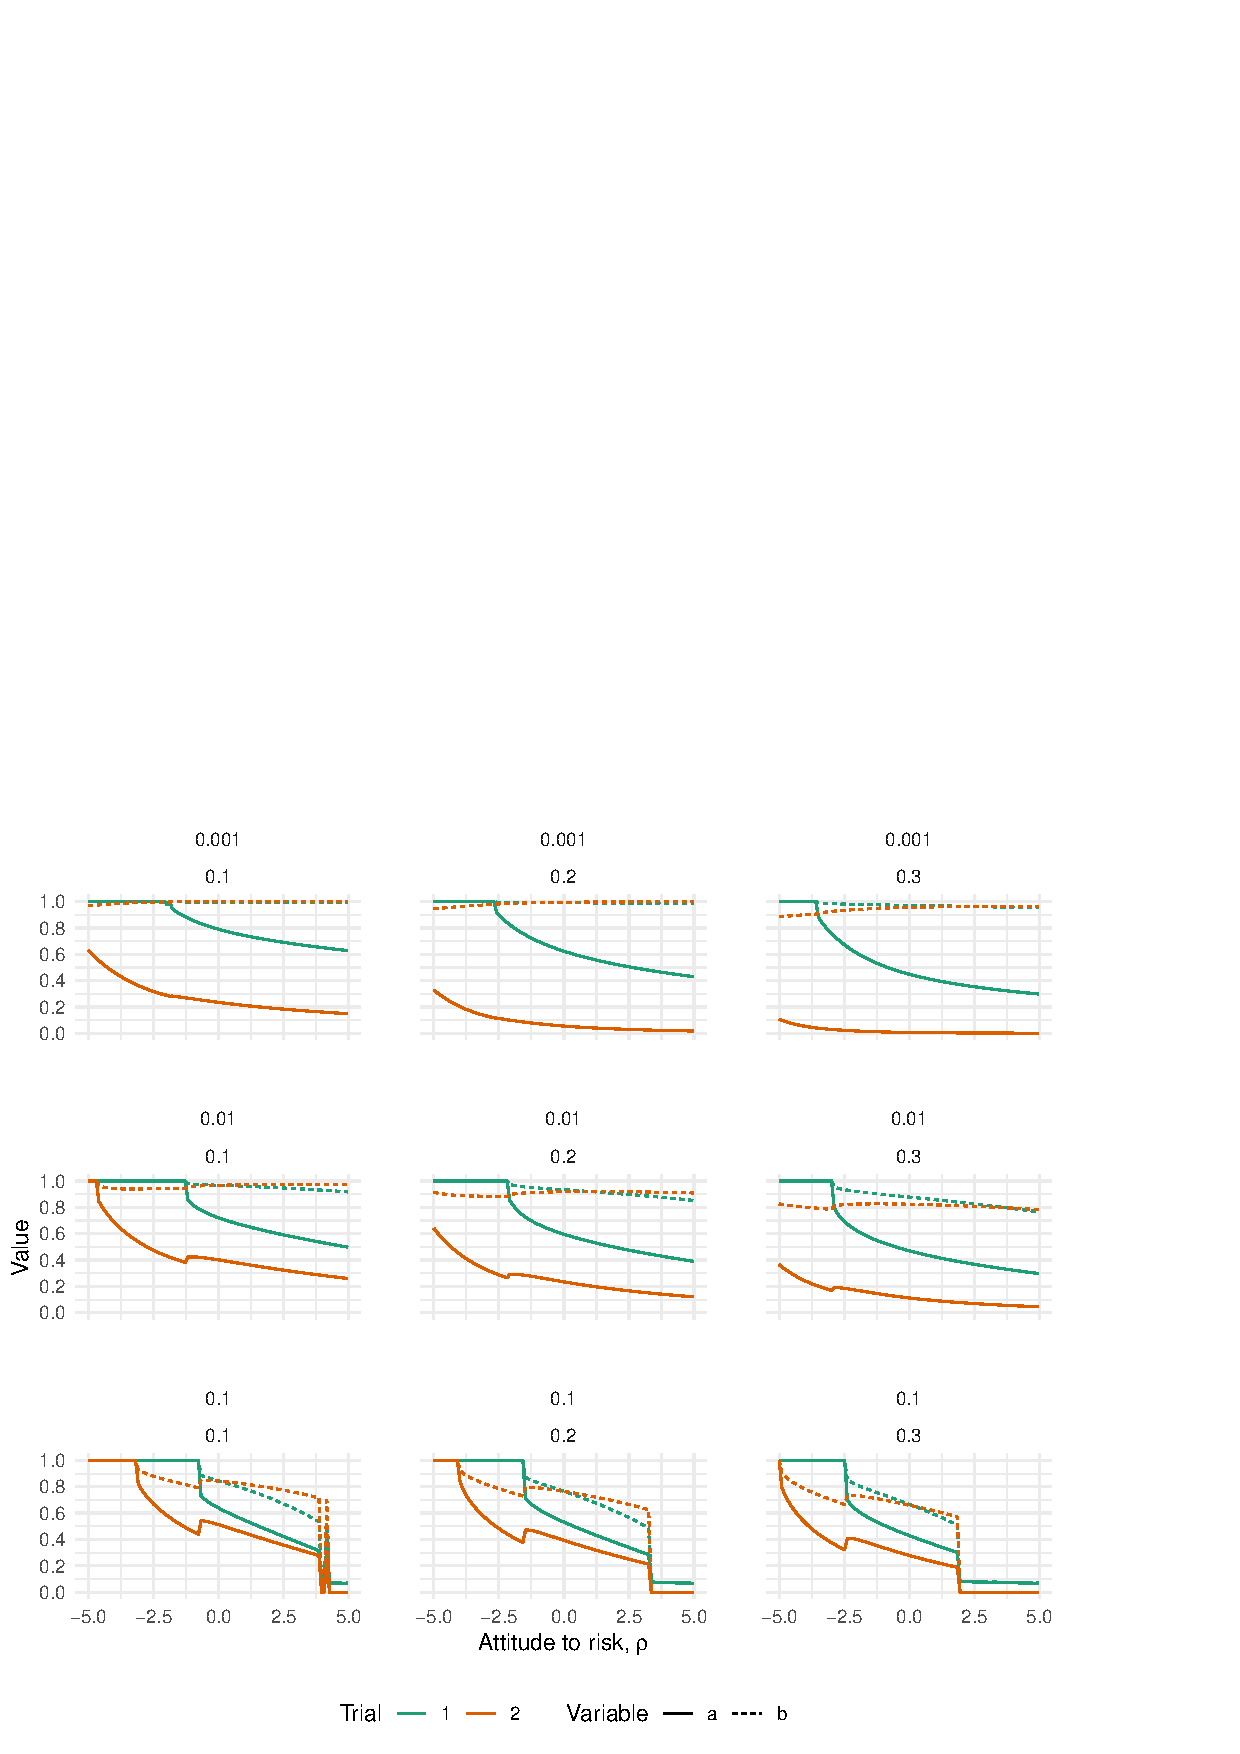
\includegraphics[scale=0.8]{./Figures/eval.pdf}
\caption{Sample sizes (dashed lines), type I error rates (solid lines) and type II error rates (dotted lines) for varying values of $\rho$ (the attitude to risk, where higher means more risk-averse) and $\bar{d}$ (the cost of sampling, where higher means a larger cost).}
\label{fig:eval}
\end{figure}

Our results show that, for the prior and treatment costs considered here, it can be optimal to not test for effectiveness in an external pilot trial. This can be seen in Figure \ref{fig:eval} where the type I error rate at stage $i=1$ reaches 1 when the attitude to risk is sufficiently risk-seeking, around $-1.25 < \rho < -2$. To understand the implications, note that $\rho = -2$ corresponds to a indifference between obtaining a treatment difference of 0.31 for certain, and a simple 50/50 gamble between obtaining a treatment difference of 0.5 or no treatment difference at all. 

In general, we find that optimal type I error rates (sample sizes) of both pilot and definitive trials decrease (increase) as we become more risk-averse, and also as the cost of sampling decreases.In terms of type II error rates of definitive trials, these \ldots

%Want to think about where it will fall down. Biggest concern would be the pilot introducing bias, probably positive, due to the idealised conditions. So, want to find optimal design when we have a bivariate normal prior on the treatment effect. Could have perfect correlation (i.e. known, fixed difference) which would give more of a sensitivity analysis; or could have a noisy relationship, which we would have to elicit. Computations are still OK - just integrating over a bivariate normal now, so can still use quadrature rules. Is there a connection here with surrogate endpoints? e.g. consider eliciting a treatment effect at 2 years, then working back to elicit the effect at two months (the pilot outcome). Need to elicit both the mean effect at each stage / outcome, but also the correlation. For correaltion, would need to ask questions like "if you found out the pilot true diff was X, what would you then think the main diff will be? Equiv to asking how much uncertainty will be left, gven estimated outcome diff. 

%Is this an evaluation of the robustness of the method, or an extension to allow fr a more general problem? More the former, but automatically provides everything we need for the latter. Put in illustration, as it's an example of how we would tackle a real problem. Define an example alternative prior and find the optimal design and compare. Want to understand how wrong using the original design would be - so measure utility diff and then translate into mu.

%In fact, this could be considered a special case of the more general issue of prior specification. So, after we get our design we might want to check if others would agree, and by how much; but crucially, we can let others use their own specific priors if we have some easy to use software.




\section{Extensions}\label{sec:extensions}

\subsection{Non-inferiority}

Although we have focussed on superiority trials, the method extends naturally to the non-inferiority setting. In a non-inferiority trial we are interested in testing whether or not the new intervention is not worse than the control by some pre-specified amount (the non-inferiority margin). The proposed method encompasses this setting by allowing for negative choices of the parameter $\hat{d}$, which denotes the amount of treatment difference we would consider equivalent to the costs of adopting the new treatment. In the non-inferiority setting the new treatment will be considered cheaper than the control, leading to a negative $\hat{d}$.

For example, if we return to the OK-Diabetes trial of Section \ref{sec:illustration} but now set $\hat{d} = -0.3$, the optimal sample size at each stage is now $n_1 = 77, n_2 = 430$. We now define type I error rate as the probability of a positive test result conditional on the non-inferiority margin $\mu = -0.5$, while power is the probability of a positive test result conditional on no difference, $\mu = 0$. The optimal design then has error rates $\alpha_1 = 0.68, \beta_1 = 0.0057, \alpha_2 = 0.034, \beta_2 = 0.0011$.


\subsection{Internal pilots}

Internal pilot trials are distinguished from external pilots by their data being used at the final analysis, with a seamless gap between the pilot and main trial stages. Extending our problem to the internal pilot setting, we continue to conduct a first test based on the pilot sample mean difference $x_1$, but now follow this with a test of the overall sample mean difference $x_t$, where
$$
x_t = \frac{n_1 x_1}{n_1 + n_2} + \frac{n_2 x_2}{n_1 + n_2}.
$$
We can now apply equation \ref{eqn:joint_cond_util} in the internal pilot by defining $G_1 = x_1 > d_1$ and $G_2 = x_t > d_2$. The relevant probabilities can be calculated by noting that the pair $x_1, x_t$, conditional on $\mu$, follow a bivariate normal distribution. Specifically, the appendix will show that
$$
\begin{pmatrix}
x_1 \\
x_t
\end{pmatrix} \mid \mu
\sim BN\left( 
\begin{pmatrix}
\mu \\
\mu
\end{pmatrix},
\begin{pmatrix}
\frac{2\sigma^2}{n_1} & \frac{2\sigma^2}{n_1 + n_2} \\
\frac{2\sigma^2}{n_1 + n_2} & \frac{2\sigma^2}{n_1 + n_2}
\end{pmatrix} \right).
$$
The probabilities in equation \ref{eqn:joint_cond_util} can now be calculated using, for example, the R package `mvtnorm' \cite{Genz2017}. Expected utility can then be calculated as before, integrating the conditional expected utility over the normal prior $p(\mu)$ using quadrature.

Applying this to the OK-Diabetes example leads to a proposed programme:

Took 16.8 mins

$n_1 = 36, n_2 = 104, \alpha_1 = 0.60, \beta_1 = 0.050, \alpha_t = 0.034, \beta_t = 0.186$

Exp u -0.30755756

Note that the overall type I and II error rates are similar in both the external and internal pilot cases, but that the internal pilot utility is lower. We would expect this as a result of the correlated data (???), but note the internal pilot would not have the extra set-up costs.

% Noting that the OK-D protocol said it would go on to be an internal pilot, but without specifying the subsequent design, return to our example and look at the difference moving to an internal pilot set-up would give. 

% Add a very short application, e.g. returing to the illustrative example and comparing the optimal designs resulting from internal and external pilot designs (expecting some kind of efficiency saving from the former, so maybe better error rates or lower sample size). Might also wantto report results differently, with an emphasis on the overall error rates of the full programme, and possibly constrtain these at fixed values and find the optimal error split between the first and second stage tests.

\subsection{Binary endpoint}

Suppose we have a binary primary endpoint, with probability of occurrence of $\tau_C$ in the control arm and $\tau_I$ in the intervention arm, and that we are interested in the absolute difference $\mu = \tau_C - \tau_I$ (interested in the sense that this is what features in our utility). We use Beta priors to reflect our prior uncertainty, with $\tau_C \sim Beta(a_C, b_C)$ and $\tau_I \sim Beta(a_I, b_I)$. We can extend our approach to this scenario by returning to equation \ref{eqn:joint_cond_util} and noting that, now conditioning on the pair of probabilities $(\tau_C, \tau_I)$, the probabilities of test success/failure at each stage can still be easily calculated. Now, rather than integrating the conditional expectation over a single normal prior density, we must integrate over the two independent beta distributions for $(\tau_C, \tau_I)$. Unable to use Gauss-Hermite quadrature, we can instead use more general numerical integration methods such as the adaptive procedure implemented in the R package `cubature' \cite{Narasimhan2018}. This is slower by a factor of $10^3$, suggesting the time needed to solve the optimisation problem will be around 15 minutes.

\subsection{Unknown variance}

When the variance of the primary outcome is unknown but still assumed to be common across arms, the tests at each stage of the design will compare $t$-statistics
$$
t_i = \frac{x_i}{\sqrt{2\hat{\sigma_i}^2 / n_i}}
$$
for stage $i = 1,2$, incorporating pooled estimates of the variance, $\hat{\sigma_i}^2$. Conditional on $\mu, \sigma^2$, these $t$-statistics will follow non-central $t$-distributions with $2n_i - 2$ degrees of freedom and non-centrality parameter $\mu/\sqrt{2\sigma^2 / n_i}$. The of test success/failure at each stage in equation \ref{eqn:joint_cond_util} (now conditioning on $\mu$ and $\sigma^2$) can then be readily calculated. Given this conditional utility, we can proceed as before by numerically integrating over the prior distribution, now a joint prior $p(\mu, \sigma^2)$. As in the case of a binary endpoint, we can use a numerical method like the `cubature' package for this integration, noting again that computation time will be increased.

%\subsection{Surrogate endpoints} We have assumed throughout that the endpoints at both stages are the same. Say we want to relax this, e.g. have the same continuous endpoint but measured earlier at the pilot stage. Closely related to the sensitivity analysis we do in the illustration, where we considered a positive bias in the pilot effect (but with the same endpoint at the same time). Key thing is that we need to elicit a bivariate distribution for the effect at both stages and the correlation between them. If we can do this, we can still use quadrature and everything will follow.

%\subsection{Two definitive trials} The FDA require as standard two statistically significant results from two different phase III trials for an intervention to be approved. If these are done simultaneously, assuming their optimal design is equal, can we modify our formulation? Same design parameters, same utility, but and additional set of trial realisation outcomes. Just need to change how we define stage 2 success $G_2$ - conditional on $\mu$, still easy to calculate (independent normals).

% Not considered for extensions here - multiple arms and multiple endpoints.

\section{Discussion}\label{sec:discussion}

% Summary and main implications
We have explored how Bayesian statistical decision theory can be used to define optimal type I and II error rates for trial programmes involving a pilot trial and subsequent definitive trial. We have introduced a general utility function, outlining the associated assumptions which it implies, and demonstrated how its parameter values can be determined. In particular, we have included in our formulation a parameter which encapsulates the attitude to risk of the decision maker, and found that optimal programme designs can be sensitive to its value. This can be contrasted with related work proposing a decision-theoretic approach to optimal trial trial design, which typically assumes a risk-neutral attitude. When evaluating the conventional approach to pilot trial analysis whereby efficacy is not tested, we found that this can be the optimal course of action but only when the decision maker is risk-seeking. As we might expect such an attitude to be rare in practice, we can conclude that efficacy should be tested in pilot trials in order to maximise utility.

% Assumptions
- Assumed normal endpoint. Extended to binary, not to time to event.
- Assumed shared endpoint. Not considered surrogacy.
- Assumed a normal prior on effectiveness. Extended (binary and unknown sd). Can generalise further with more complicated integration; MC could always be used, but optimisation could be slow (only need to sample once though, so just need a fast vectorised objective function).
- Assumed three specific attributes.  Did not allow for more than one substantive parameter, e.g. no safety param. 
- Did not include set-up costs, but could do easily if quantified in terms of sampling. Should only affect cases where we now might not want to do a trial at all.
- Did not model take-up of treatment, e.g. no finite patient horizon as in \cite{Pearce2018} and others. 
- Assumed mutual preference independence between attributes. 
- Assumed linear individual value functions.
- Require the decision-maker to answer three elicitation questions for utility; but have shown how a sensitivity analysis can explore how robust the locally optimal design is.
- Assumed utility independence of d over the other attributes.

% Extending to other scenarios



We have considered programmes where a hypothesis test is used in the primary analysis of the pilot and definitive trials. Further work could consider allowing for a Bayesian analysis at one or both stages. In particular, it would be of interest to explore how a Bayesian analysis of pilot trial data could be used to update prior beliefs and use the revised knowledge to optimise the subsequent definitive trial. For example, value of information methods could be used to determine the definitive trial's sample size \cite{Willan2005}. A potential difficulty with such an approach is the computational aspect of such calculations, although techniques for enabling fast calculation may be useful in this regard\cite{Strong2015}. 

We have focussed on using pilot trials to test the efficacy of the intervention. Typically, pilot trials are used to estimate other parameters relating to the feasibility of the definitive trial, such as recruitment, follow-up and adherence rates \cite{Avery2017}.



Alternative frameworks for choosing optimal error rates - minimising a weighted sum of the two types; adaptive designs which, given an overall nominal rate (arbitrarily chosen), will lead to optimal pilot OCs; fixing at some other (arbitrary) value like 0.5 in \cite{Cocks2013}.

Alternatives to pilot design, outwith an N-P testing convention - full Bayes decision-theoretic approach, making decisions at the end of each stage to maximise utility, making design choices (sample size) based on expected value of sample information; using the stage 1 results to inform the stage two design, e.g. by updating the prior;

Using the method in practice - eliciting subjective priors; eliciting utility function parameters; incorporating several decision-makers with different views;

Recall that we assumed identity value functions for the three attributes only to avoid cluttering the notation. We can simply replace the terms with the proper value functions and the general method will still hold. Thus, we can include situations where, for example, there is a concave value function on change in primary outcome (less benefit accruing as it increases). More generally, need to give people an idea of what they can change. So, can remove anything trivially. Can add deterministic attributes whose value depend only on the test results, e.g. set-up costs, trivially. Can't add attributes with uncertain parameters without a more thoughtful extension. Can generalise the utility we have by using non-identity value functions but keeping the additive form - so maintaining the same assumptions about preference independence etc. If we don't have preference independence we would need multi-linear or nonlinear value functions, wouldn't have the exponential utility result, and would need a much more involved elicitation process.



\begin{acks}
Acknowledgements.
\end{acks}

\begin{dci}
The Authors declare that there is no conflict of interest.
\end{dci}

\begin{funding}
This work was supported by the Medical Research Council [grant number MR/N015444/1].
\end{funding}

\bibliographystyle{SageV}
\bibliography{C:/Users/meddwilb/Documents/Literature/Databases/DTWrefs}

\section*{Appendix}

\subsection*{Expected utility for a single trial}

The utility function is $u(\mu, x)$, where $\mu$ is the true difference and $x$ is the sample mean difference. Note that
$$
x \mid \mu \sim N\left(\mu, \frac{2\sigma^2}{n} \right).
$$
Given a normal prior $\mu \sim N(\mu_0, \sigma_0^2)$, the posterior distribution of $\mu$ is also normal. Specifically
$$
\mu \mid x \sim N \left( \mu_1 = \sigma_1^2 \left( \frac{\mu_0}{\sigma_0^2} + \frac{xn}{2\sigma^2} \right), ~ \sigma_1^2 = 1/\left( \frac{1}{\sigma_0^2} + \frac{n}{2\sigma^2} \right) \right).
$$
The marginal distribution of the sample mean difference is
$$
x \sim N\left(\mu_0, \sigma_x^2 = \sigma_0^2 + \frac{2\sigma^2}{n} \right).
$$

For the case $\rho = 0$, the utility function is the value function. The expected utility is then
\begin{align*}
E[u(\mu, x)] =& E_x\left[ E_{\mu | x} [u(\mu, x)] \right] \\
=& E_x \left[ I\{x > d\} (k_d \mu_1 + k_n n) + I\{x \leq d\} (k_n n + k_c) \right] \\
=& k_n n + Pr(x > d) k_d E_{x | x > d} \left[ \mu_1 \right] + Pr(x \leq d)k_c,
\end{align*}
The two probabilities follow from the marginal distribution of the sample mean. For example,
$$
Pr[x > d] = 1- \Phi\left(\frac{d-\mu_0}{\sqrt{\sigma_0^2 + \frac{2\sigma^2}{n}}} \right)
$$
The expectation is of $\mu_1$, the mean of the posterior distribution on $\mu$ given $x$, with respect to the distribution of $x$ conditional on $x > d$. This is a truncated normal with mean
$$
E_{x | x > d} \left[ \mu_1 \right] = \mu_0 + \sigma_x \phi\left(\frac{d - \mu_0}{\sigma_x} \right)/\left(1 - \Phi\left(\frac{d - \mu_0}{\sigma_x}\right) \right).
$$

For the case $\rho > 0$, we again start with the law of total expectation giving $E[u(\mu, x)] = E_x\left[ E_{\mu | x} [u(\mu, x)] \right]$. Then,
\begin{align*}
E_{\mu | x} [u(\mu, x)] &= E_{\mu | x}[1 - e^{-\rho(k_d\mu + k_n n) I\{x > d\} -\rho(k_n n + k_c) I\{x < d\}}] \\
&= I\{x > d\} E_{\mu | x}[1 - e^{-\rho(k_d\mu + k_n n)}] + I\{x < d\}E_{\mu | x}[1 - e^{-\rho(k_n n + k_c)}]
\end{align*}
For the first term we have:
$$
E_{\mu | x}[1 - e^{-\rho(k_d\mu + k_n n)}] = 1 - e^{-\rho k_n n} E_{\mu | x}[e^{-\rho k_d \mu}]
$$
This takes the form as a moment generating function: for a normally distributed $Y \sim N(a, b^2)$,
$$
E[e^{tY}] = e^{ta + \frac{b^2 t^2}{2}}.
$$
This gives us
$$
E_{\mu | x}[1 - e^{-\rho(k_d\mu + k_n n)}] = 1 - e^{-\rho k_n n} \left(e^{t\mu_1 + \frac{\sigma_1^2 t^2}{2}} \right),
$$
where $t = \rho k_d$. This then all gives an expected utility conditional on $x$ of
$$
E_{\mu | x} [u(\mu, x)] = I\{x > d\} \left[1 - e^{-\rho k_n n} \left(e^{t\mu_1 + \frac{\sigma_1^2 t^2}{2}} \right) \right] + I\{x < d\}\left[1 - e^{-\rho(k_n n + k_c)}\right].
$$
We now need to take the expectation of this over the marginal distribution for $x$:
$$
\begin{aligned}
E[u(\mu, x)] &= E_x\left[ E_{\mu | x} [u(\mu, x)] \right] \\
 &= E_x\left[ I\{x > d\} \left(1 - e^{-\rho k_n n} e^{t\sigma_1^2(\frac{\mu_0}{\sigma_0^2} + \frac{xn}{2\sigma^2}) + \frac{\sigma_1^2 t^2}{2}} \right) \right] + 
 E_x\left[ I\{x < d\}\left(1 - e^{-\rho(k_n n + k_c)}\right) \right].
\end{aligned}
$$
The first term is equal to
$$
Pr[x > d] \left( 1 - e^{-\rho k_n n} e^{\frac{\sigma_1^2 t^2}{2}} e^{\frac{t\sigma_1^2 \mu_0}{\sigma_0^2}}   \right) E_x \left[ e^{\frac{t\sigma_1^2 x n}{2\sigma^2}} \right].
$$
For the expectation, we again use a moment generating function. Here, the sample difference $x$ is normally distributed $N(\mu_0, \sigma_x^2)$ but we have conditioned on $x > d$ and so have a truncated normal. The moment generating function for $Y \sim N(a,b^2), Y > d$ is
$$
E[e^{rY}] =  \left( e^{ar + \frac{b^2 r^2}{2} } \right) \left(\frac{1 - \Phi(\frac{d-a}{b} - br)}{1 - \Phi(\frac{d-a}{b} )} \right)
$$
So, for our case we have
$$
 E_x \left[ e^{\frac{t\sigma_1^2 x n}{2\sigma^2}} \right] = \left( e^{\mu_0 r + \frac{\sigma_x^2 r^2}{2} } \right) \left(\frac{1 - \Phi(\frac{d-\mu_0}{\sigma_x} - \sigma_x r)}{1 - \Phi(\frac{d-\mu_0}{\sigma_x})} \right),
$$
where $r = \frac{t \sigma_1^2 n}{2\sigma^2}$. Finally, putting everything together, we get
\begin{align*}
E[u(\mu, x)] =& E_x\left[ E_{\mu | x} [u(\mu, x)] \right] \\
 =& \left[ 1- \Phi\left(\frac{d-\mu_0}{\sqrt{\sigma_0^2 + \frac{2\sigma^2}{n}}} \right)  \right] \left[ 1 - e^{-\rho k_n n} e^{\frac{\sigma_1^2 t^2}{2}} e^{\frac{t\sigma_1^2 \mu_0}{\sigma_0^2}} \left( e^{\mu_0 r + \frac{\sigma_x^2 r^2}{2} } \right) \left(\frac{1 - \Phi(\frac{d-\mu_0}{\sigma_x} - \sigma_x r)}{1 - \Phi(\frac{d-\mu_0}{\sigma_x})} \right)  \right] + \\
 & \Phi\left(\frac{d-\mu_0}{\sqrt{\sigma_0^2 + \frac{2\sigma^2}{n}}} \right) \left[1 - e^{-\rho(k_n n + k_c)}\right].
\end{align*}
The case $\rho < 0$ follows immediately.

\subsection*{Internal pilot sampling distribution}

Recall that we have sample means from both the first and second stage of an internal pilot design, $x_1, x_2$, with the combined sample mean $x_t = \frac{n_1 x_1}{n_1 + n_2} + \frac{n_2 x_2}{n_1 + n_2}$ being used at the final testing stage. The distribution of the combined mean, conditional on $\mu$ is $x_t \mid \mu \sim N\left( \mu, \frac{2\sigma^2}{n_1 + n_2} \right)$. To fully specify the joint distribution of $(x_1, x_t)$ we require the covariance:
$$
cov(x_1, x_t) = E[x_1 x_t] - E[x_1] E[x_t].
$$
By the law of total expectation,
\begin{align*}
E[x_1 x_t] &= E_{x_1} ( E_{x_1 x_t | x_1}[x_1 x_t] ) \\
&= E_{x_1} ( x_1 E_{x_t | x_1}[x_t] ) \\
&= E_{x_1} \left( x_1 E_{x_t | x_1}\left[\frac{n_1 x_1}{n_1 + n_2} + \frac{n_2 x_2}{n_1 + n_2}\right] \right) \\
&= E_{x_1} \left( \frac{n_1 x_1^2}{n_1 + n_2} + \frac{n_2 x_1 \mu}{n_1 + n_2} \right) \\
&= \frac{n_1}{n_1 + n_2} E[x_1^2] + \frac{n_2}{n_1 + n_2} E[x_1] \mu \\
&= \frac{n_1}{n_1 + n_2} (var(x_1) + E[x_1]^2) + \frac{n_2}{n_1 + n_2} \mu^2 \\
&= \frac{n_1}{n_1 + n_2} \left(\frac{2\sigma^2}{n_1} + \mu^2\right) + \frac{n_2}{n_1 + n_2} \mu^2.
\end{align*}
Then,
\begin{align*}
cov(x_1, x_t) &= \frac{n_1}{n_1 + n_2} \left(\frac{2\sigma^2}{n_1} + \mu^2\right) + \frac{n_2}{n_1 + n_2} \mu^2 - \mu^2 \\
&= \frac{2\sigma^2}{n_1 + n_2} + \frac{n_1 \mu^2}{n_1 + n_2} + \frac{n_2 \mu^2}{n_1 + n_2} - \mu^2 \\
&= \frac{2\sigma^2}{n_1 + n_2} .
\end{align*}


\end{document}

\subsection*{Partial derivatives of expected utility}

Denoting $Pr[G_i = 1 ~|~ \mu] = Pr[x_i > d_i 1 ~|~ \mu] = g(n_i, d_i)$ and $Pr[G_i = 0 ~|~ \mu] = Pr[x_i \leq d_i 1 ~|~ \mu] = \bar{g}(n_i, d_i)$ we can re-write the conditional expected utility of equation \ref{eqn:joint_cond_util} as
$$
\begin{aligned}
f(n_1,n_2,d_1,d_2) = &g(n_1,d_1)g(n_2,d_2) - g(n_1,d_1)g(n_2,d_2)\exp(-\rho(k_d\mu + k_n (n_1+n_2)) +\\
&g(n_1,d_1)\bar{g}(n_2,d_2) - g(n_1,d_1)\bar{g}(n_2,d_2)\exp(-\rho(k_n (n_1+n_2) + k_c)) + \\
&\bar{g}(n_1,d_1) - \bar{g}(n_1,d_1)\exp(-\rho(k_n n_1 + k_c)).
\end{aligned}
$$
Then, using the partial derivatives
$$
\frac{d}{dn_i} g(n_i,d_i) = \frac{d}{dn_i} \left[1 - \Phi \left(\frac{d_i-\mu}{\sqrt{2\sigma^2/n_i}} \right)\right] = -\phi\left(\frac{d_i-\mu}{\sqrt{2\sigma^2/n_i}} \right) \frac{d_i-\mu}{2\sqrt{2\sigma^2/n_i}}
$$
and
$$
\frac{d}{dd_i} g(n_i,d_i) = \frac{d}{dd_i} \left[1 - \Phi \left(\frac{d_i-\mu}{\sqrt{2\sigma^2/n_i}} \right)\right] = -\phi\left(\frac{d_i-\mu}{\sqrt{2\sigma^2/n_i}} \right) \frac{1}{\sqrt{2\sigma^2/n_i}},
$$
we can calculate the partial derivatives of the integrand in equation \ref{eqn:exp_util}. Given the quadrature approximation being used, the partial derivatives of the expected utility can then be calculated as the weighted sum of derivatives at the quadrature points. Full details can be found in the supplementary material.
